\subsection{Quark/gluon and $W$ tagging}

Samples were generated at $\sqrt{s} = 8\TeV$ for QCD dijets, and for $W^+W^-$
pairs produced in the decay of a (pseudo) scalar resonance and
decaying hadronically. The QCD events
were split into subsamples of $gg$ and $q\bar{q}$ events, allowing for tests of
discrimination of hadronic $W$ bosons, quarks, and gluons.

Individual $gg$ and $q\bar{q}$ samples were produced at leading order (LO)
using \textsc{MadGraph5}, while $W^+W^-$ samples were generated using
the \textsc{JHU Generator} to allow for separation of longitudinal and
transverse polarizations. Both were generated using \textsc{CTEQ6L1}
PDFs\refneeded. The samples were produced in exclusive $p_T$ bins
of width 100 {\GeV}, with the slicing parameter
chosen to be the $p_T$ of any final state parton or $W$ at LO. At the
parton-level the \pt bins investigated were 300-400 GeV, 500-600 GeV
and 1.0-1.1 TeV. Since
no matching was performed, a cut on any parton was equivalent. The samples were
then all showered through \textsc{Pythia8} (version 8.176) using the default tune 4C.

The showered events were clustered with \textsc{FastJet}
3.03\refneeded using
the \antikt~algorithm\refneeded with jet radii of $R = 0.4,\, 0.8,\, 1.2$. In
both signal and background, an upper and lower cut on
the leading jet $\pt$ is applied after showering/clustering, to ensure
similar $\pt$ spectra for signal and background in each \pt~bin. The bins
in leading jet \pt that are investigated in the W-tagging and
q/g tagging studies are 300-400 GeV, 500-600 GeV, 1.0-1.1 TeV. The
distribution of the leading jet \pt~for the $gg$ and $WW$ samples in
the 300-400 GeV parton \pt~slice prior to the requirement on the
leading jet \pt~is shown in Figure~\ref{fig:pt300_basics}, for the
R=0.8 and R=1.2 \antikt~jet radii considered in this
\pt~slice. Figures~\ref{fig:pt500_basics} and~\ref{fig:pt1000_basics}
show the equivalent leading jet \pt~distributions for the jet radii
considered in the 500-600 GeV and 1.0 - 1.1 TeV slices respectively.

\begin{figure*}
\begin{center}
\subfigure[\antikt R=0.8]{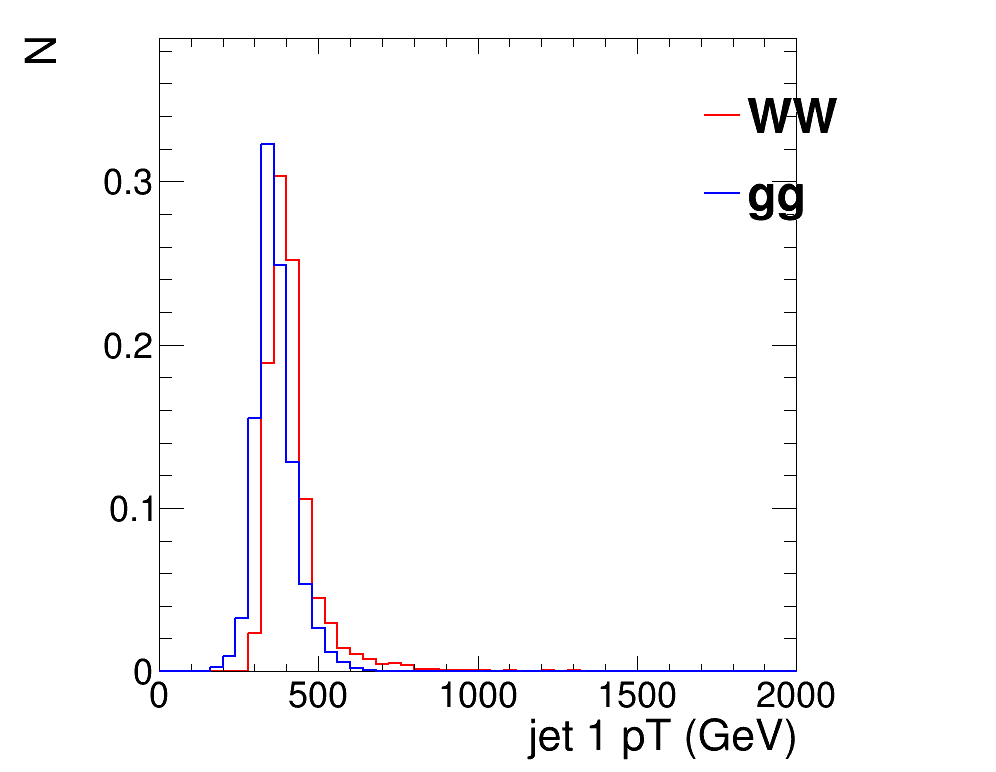
\includegraphics[width=0.30\textwidth]{./Figures/WTagging/pT300/AKtR08/jpt1.png}}
\subfigure[\antikt R=1.2]{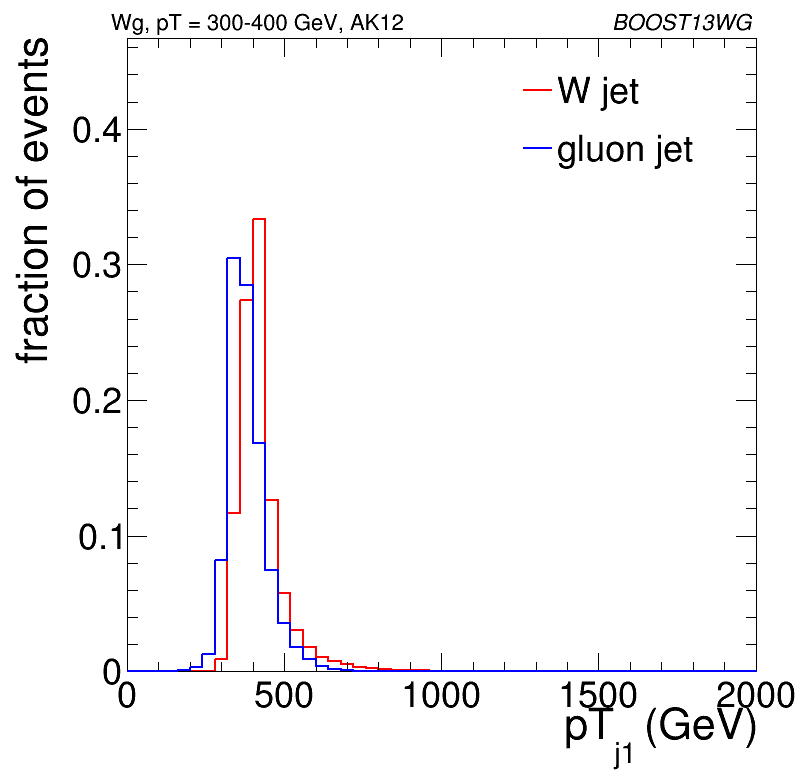
\includegraphics[width=0.30\textwidth]{./Figures/WTagging/pT300/AKtR12/jpt1.png}}
\caption{Comparisons of the leading jet \pt spectrum of the $gg$
  background to the $WW$ signal in the \pt 300-400 GeV parton \pt~slice using the
  different \antikt jet distance parameters explored in this \pt~bin. These
  distributions are formed prior to the 300-400 GeV leading jet \pt~requirement.}
\label{fig:pt300_basics}
\end{center}
\end{figure*}

\begin{figure*}
\begin{center}
\subfigure[\antikt R=0.8]{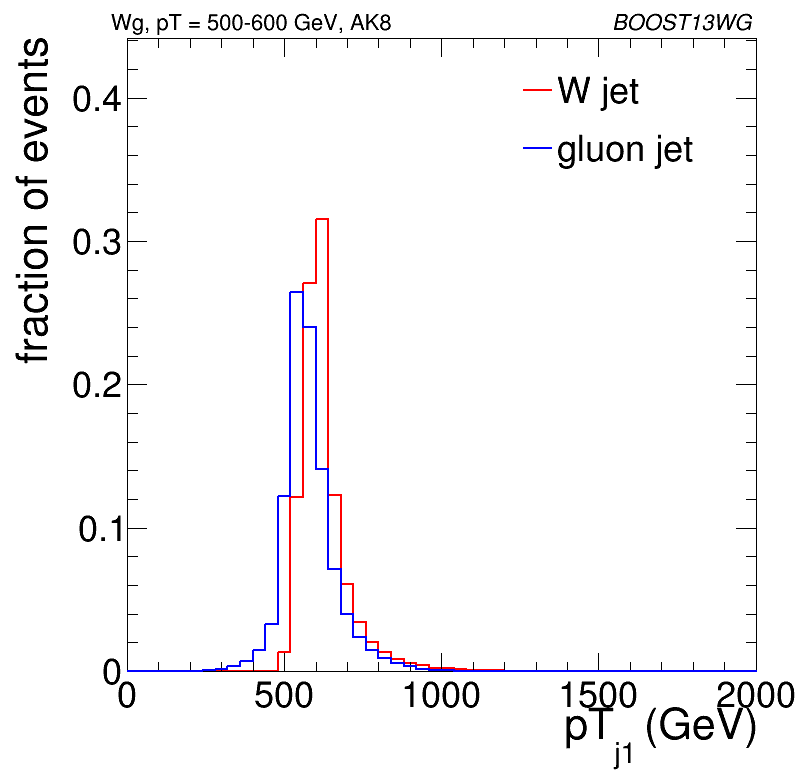
\includegraphics[width=0.30\textwidth]{./Figures/WTagging/pT500/AKtR08/jpt1.png}}
\subfigure[\antikt R=1.2]{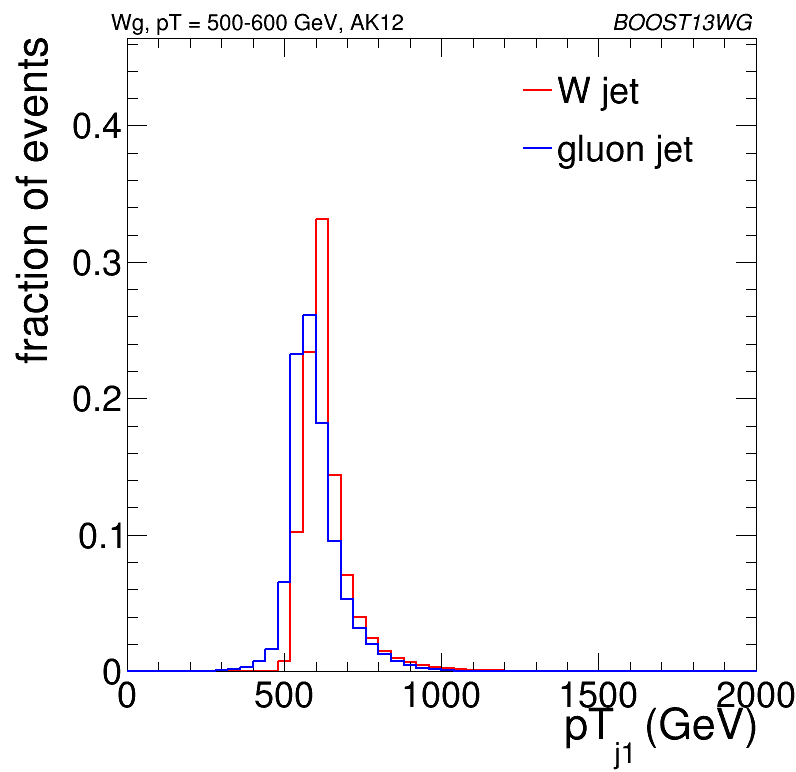
\includegraphics[width=0.30\textwidth]{./Figures/WTagging/pT500/AKtR12/jpt1.png}}
\caption{Comparisons of the leading jet \pt spectrum of the $gg$
  background to the $WW$ signal in the \pt 500-600 GeV parton \pt~slice using the
  different \antikt jet distance parameters explored in this \pt~bin. These
  distributions are formed prior to the 500-600 GeV leading jet \pt~requirement.} 
\label{fig:pt500_basics}
\end{center}
\end{figure*}

\begin{figure*}
\begin{center}
\subfigure[\antikt R=0.4]{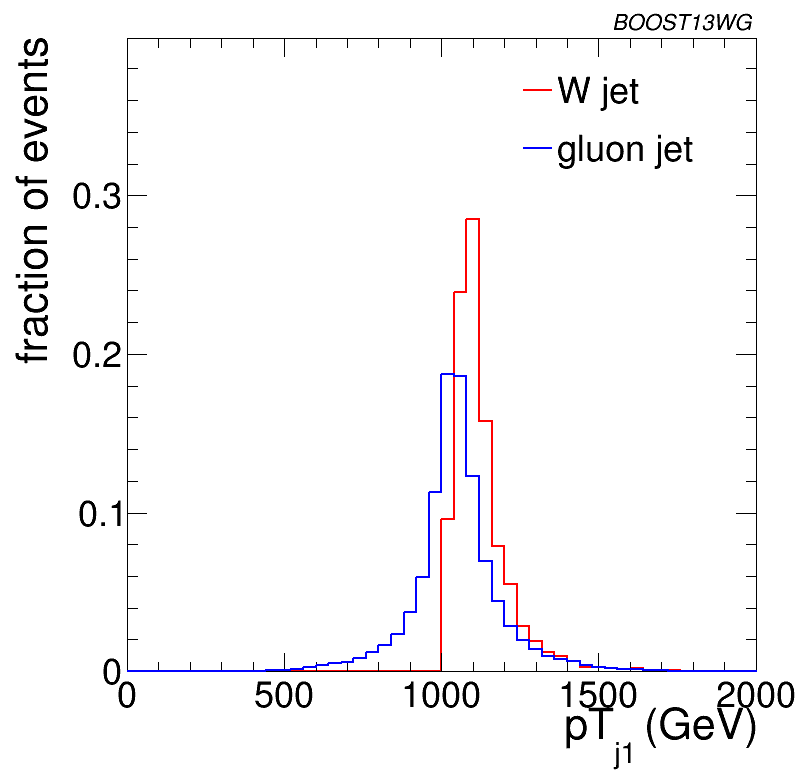
\includegraphics[width=0.30\textwidth]{./Figures/WTagging/pT1000/AKtR04/jpt1.png}}
\subfigure[\antikt R=0.8]{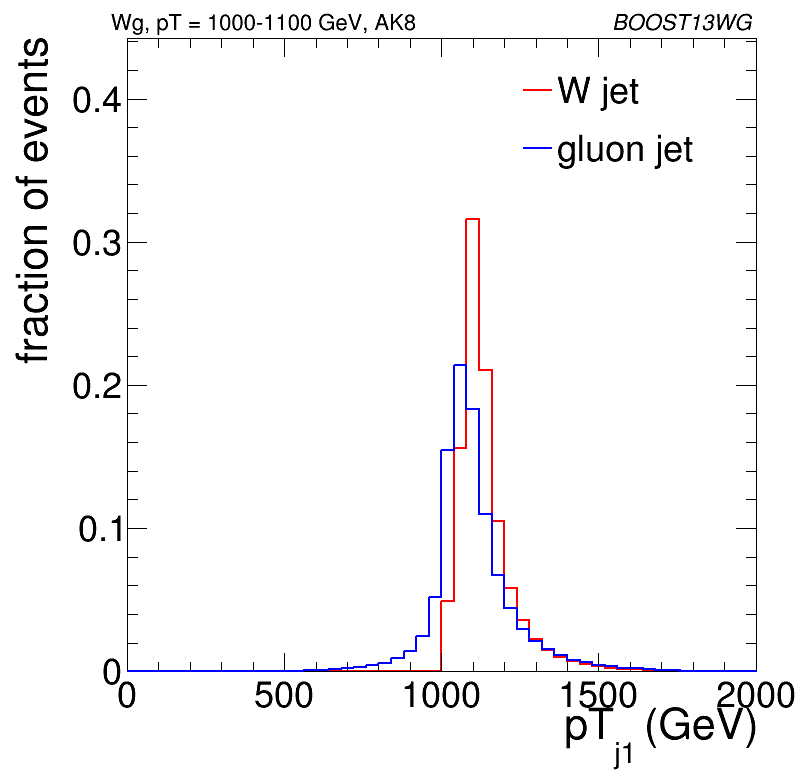
\includegraphics[width=0.30\textwidth]{./Figures/WTagging/pT1000/AKtR08/jpt1.png}}
\subfigure[\antikt R=1.2]{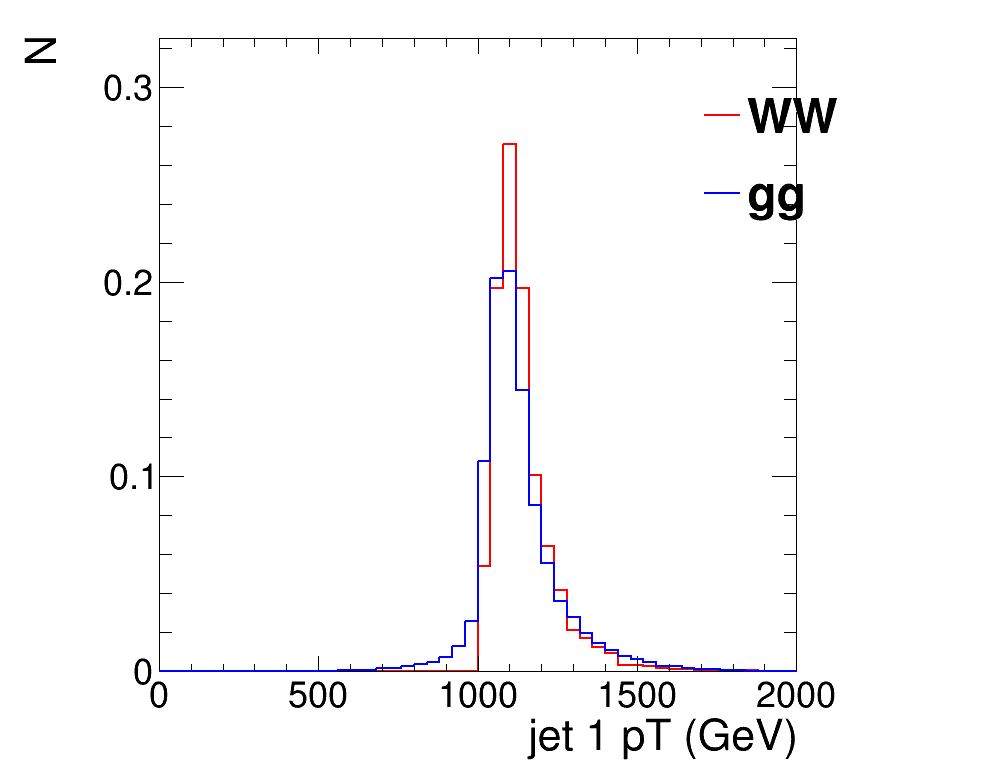
\includegraphics[width=0.30\textwidth]{./Figures/WTagging/pT1000/AKtR12/jpt1.png}}
\caption{Comparisons of the leading jet \pt spectrum of the $gg$
  background to the $WW$ signal in the \pt 1.0-1.1 TeV parton \pt~slice using the
  different \antikt jet distance parameters explored in this \pt~bin. These
  distributions are formed prior to the 500-600 GeV leading jet \pt~requirement.}
\label{fig:pt1000_basics}
\end{center}
\end{figure*}


\subsection{Top tagging}
Samples were generated at $\sqrt{s}=14\TeV$. Standard Model dijet and top pair
samples were produced with \textsc{Sherpa} 2.0.0\refneeded, with matrix elements of up
to two extra partons matched to the shower. The top samples included only
hadronic decays and  were generated in exclusive $\pt$ bins of width 100 \GeV,
taking as slicing parameter the maximum of the top/anti-top $\pt$. The QCD
samples were generated with a cut on the leading parton-level jet $\pt$, where
parton-level jets are clustered with the anti-$k_t$ algorithm and jet radii of
$R= 0.4,\,0.8,\,1.2$. The matching scale is selected to be $Q_{\rm cut}=40, 60, 80 \GeV$ for
the $p_{T\,\text{min}}=600, 1000$, and $1500 \GeV$ bins, respectively.
 
The analysis again relies on \textsc{FastJet} 3.0.3 for jet clustering and
calculation of jet substructure observables, and an upper and lower $\pt$ cut are applied
to each sample to ensure similar $\pt$ spectra in each bin. The bins in leading jet $\pt$
that are investigated for top tagging are 600-700 GeV, 1-1.1 TeV, and
1.5-1.6 TeV. {\bf ED: What jet algorithm is used to define the \pt~bins?}